\documentclass[12pt,letterpaper,fleqn]{hmcpset}
\usepackage[margin=1in]{geometry}
\usepackage{graphicx}

% info for header block in upper right hand corner
\name{Lan Fangzhou}
\class{Pattern-Recognizing}
\assignment{Assignment-2}
\duedate{}

\begin{document}

\problemlist{03-Framework.pdf.1, 04-Error.pdf.2, 04-Error.pdf.5, 04-Error.pdf.7, 05-PCA.1, 05-PCA.2, 05-PCA.3}

\begin{problem}[03-Framework.pdf.1]
\end{problem}
\begin{solution}
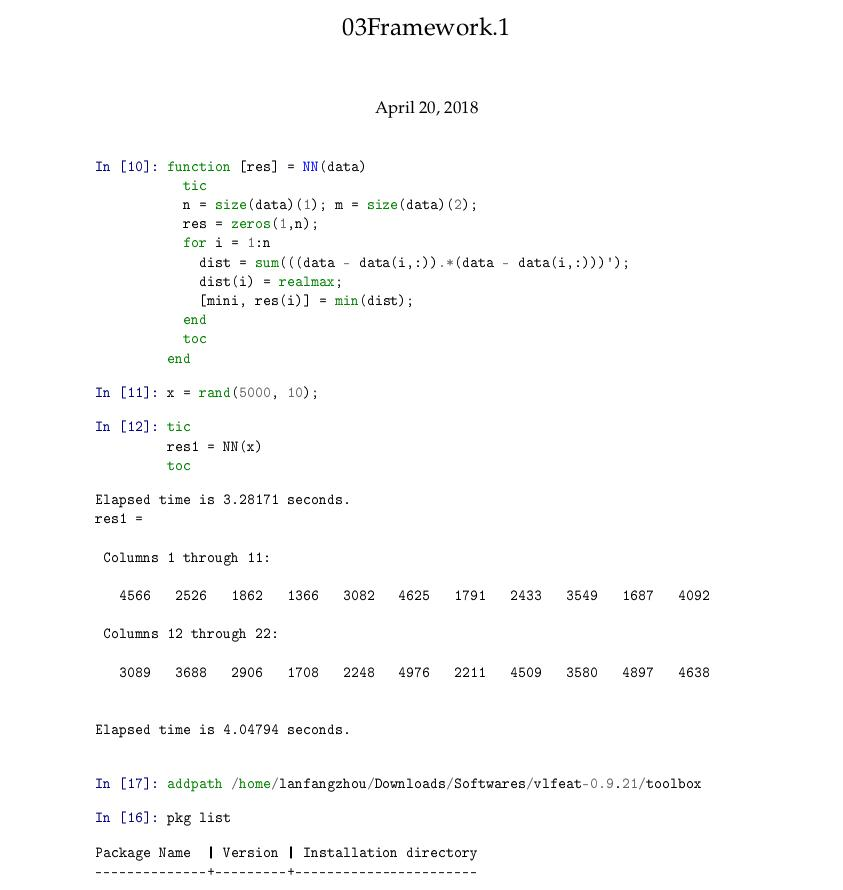
\includegraphics[width=1\textwidth]{10.jpg}\\
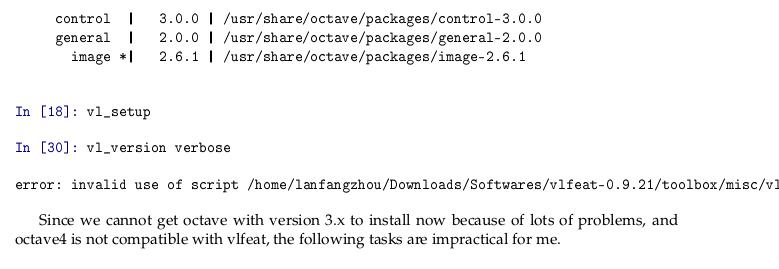
\includegraphics[width=1\textwidth]{11.jpg}\\
\end{solution}

\begin{problem}[04-Error.pdf.2]
\end{problem}
\begin{solution}
(a)
\begin{align*}
\text{find $\beta \in R^d$ to minimize }\sum_{i=1}^{n}(y_i-x_i^T\beta)^2
\end{align*}
(b)
\begin{align*}
\text{find $\beta \in R^d$ to minimize }(y-X\beta)^T(y-X\beta)
\end{align*}
(c)
\begin{align*}
&\text{We first calculate the derivative of the objective}\\
&\frac{d((y-X\beta)^T(y-X\beta))}{d\beta}=-2X^T(y-X\beta)\\
&\text{Let it = 0 :}\\
&\beta=(X^TX)^{-1}X^Ty\\
&\text{Which is the optimal value.}
\end{align*}
(d)
\\No. When $d>n$, $rank(X^TX)\le rank(X)=d<n=size(X^TX)$
\\\\(e)
\\The regularizer will decrease the $norm_2$ of $\beta$, i.e, decrease the magnitude of $\beta$.
\\\\(f)
\begin{align*}
&\text{find $\beta \in R^d$ to minimize }(y-X\beta)^T(y-X\beta)+\lambda\beta^T\beta\\
&\text{We first calculate the derivative of the objective}\\
&\frac{d((y-X\beta)^T(y-X\beta))+\beta^T\beta}{d\beta}=-2X^T(y-X\beta)+2\lambda\beta\\
&\text{Let it = 0 :}\\
&\beta=(X^TX+\lambda I)^{-1}X^Ty \text{ (if } X^TX+\lambda I \text{ is invertible)}\\
\end{align*}
(g)
\\The parameter $\lambda$ will make the matrix more likely to be invertible, and definitely invertible when $\lambda\to +\infty$.
\\\\(h)
\\No. For the definition of the cost function, the optimal value for $\lambda$ is when $\lambda\to 0$, which is not what we want.
\end{solution}

\begin{problem}[04-Error.pdf.5]
\end{problem}
\begin{solution}
(a)(b)
\\AUC-PR: $(r_i-r_{i-1})\frac{p_i+p_{i-1}}{2}$
\\AP: $(r_i-r_{i-1})p_i$\\\\
\begin{tabular}[t]{ccc|cccc}
\text{index} &\text{label} &\text{score} &\text{precision} &\text{recall} &\text{AUC-PR} &\text{AP}\\
\hline
0& & &1.0000&0.0000&-&-\\
1&1&1.0&1.0000&0.2000&0.2000&0.2000\\
2&2&0.9&0.5000&0.2000&0.0000&0.0000\\
3&1&0.8&0.6667&0.4000&0.1167&0.1667\\
4&1&0.7&0.7500&0.6000&0.1417&0.1333\\
5&2&0.6&0.6000&0.6000&0.0000&0.0000\\
6&1&0.5&0.6667&0.8000&0.1267&0.1333\\
7&2&0.4&0.5714&0.8000&0.0000&0.0000\\
8&2&0.3&0.5000&0.8000&0.0000&0.0000\\
9&1&0.2&0.5556&1.0000&0.1111&0.1056\\
10&2&0.1&0.5000&1.0000&0.0000&0.0000\\
\hline
& & & & &0.6962&0.7389\\
\end{tabular}
\\\\(c)
\\newAUC: 0.6907  
\\newAP: 0.7333
\\\\(d)\\
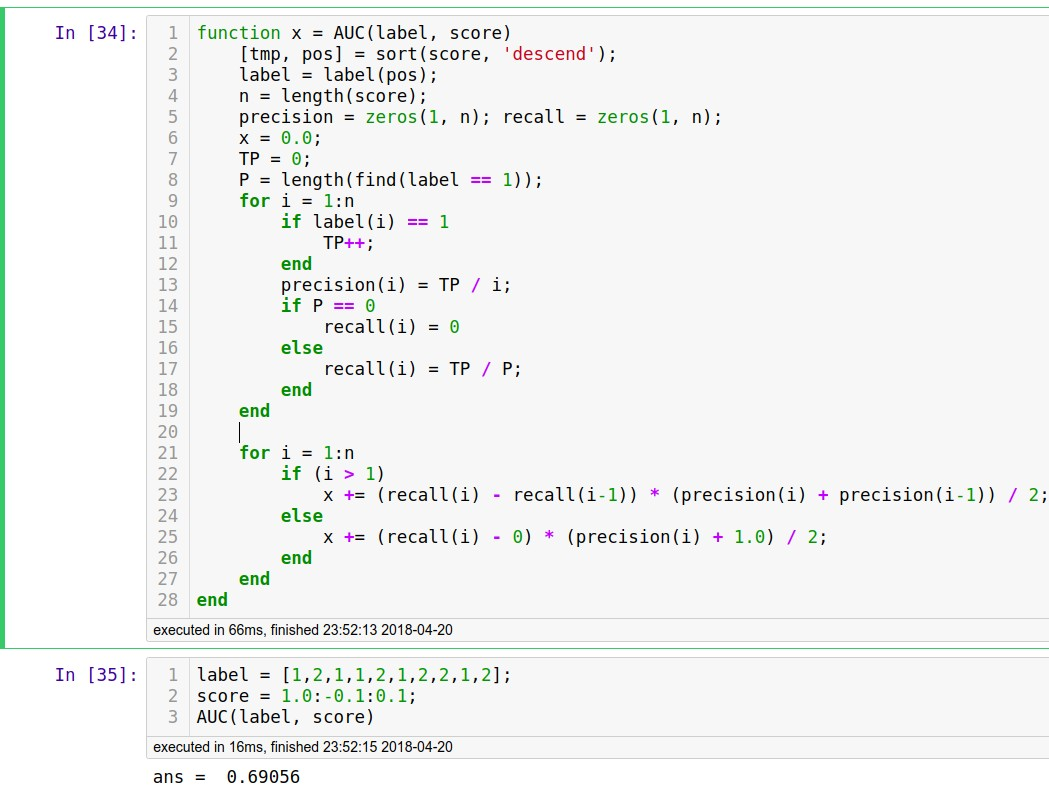
\includegraphics[width=1\textwidth]{1.jpg}
\end{solution}

\begin{problem}[04-Error.pdf.7]
\end{problem}
\begin{solution}
(a)
\\
$$p(x,y)=
\begin{cases}
0.5\cdot\frac{1}{\sqrt{2\pi}\cdot 0.5}e^{-\frac{(x+1)^2}{0.5^2}},& \text{y=1}\\
0.5\cdot\frac{1}{\sqrt{2\pi}\cdot 0.5}e^{-\frac{(x-1)^2}{0.5^2}},& \text{y=2}
\end{cases}$$
\\(b)
\\\\ $1^\circ$
\\One solution is:
\begin{align*}
f(x) &= argmax_yp(y|x)\\
&=argmax_y\frac{p(x|y)p(y)}{p(x)}\\
&=argmax_yp(x|y)\\
\end{align*}
The cost:
\begin{align*}
E_{(x,y)}[c_{y,f(x)}]&=0.5E_x[c_{1,f(x)}]+0.5E_x[c_{2,f(x)}]\\
&=0.5(Pr(f(x)=2|y=1)+Pr(f(x)=1|y=2))\\
&=0.5(\int_{f(x)=2}p(x|y=1)+\int_{f(x)\ne 2}p(x|y=2))\\
&=0.5(\int_{-\infty}^{+\infty} min(p(x|y=1),p(x|y=2))\\
&\ge 0.5(Pr(x\ge 0|y=1)+Pr(x\le 0|y=2))\\
&\text{the minimum is obtained when f(x) is set as above.}\\
&\text{Under this solution, the cost is: }\\
&=0.5(Pr(x\ge 0|y=1)+Pr(x\le 0|y=2))\\
&=2(1-\Phi(2)) \text{ ($\Phi$ is cdf of normal distribution.) }\\
&\approx 2(1-0.97725)\\
&=0.045500
\end{align*}
\\\\ $2^\circ$
\\In a multi-class classification problem, also true.
\\\\(c) 
\\Let $y = f(x) = argmax_yp(y|x)$
\\Bayes risk: 0.045500
\\\\(d)
\begin{align*}
E_{(x,y)}[c_{y,f(x)}]&=0.5E_x[c_{1,f(x)}]+0.5E_x[c_{2,f(x)}]\\
&=0.5(Pr(f(x)=2|y=1)+10Pr(f(x)=1|y=2))\\
&=0.5(\int_{-\infty}^{+\infty} min(p(x|y=1),10p(x|y=2))\\
\end{align*}
\indent \indent Thus$$f(x)=
\begin{cases}
1,&p(x|y=1)\ge 10p(x|y=2)\\
2,&p(x|y=1)<10p(x|y=2)
\end{cases}$$
\end{solution}

\begin{problem}[05-PCA.1]
\end{problem}
\begin{solution}
(a)
\\Since $U,V$ are orthogonal:
\\$XX^T=(U\Sigma V^T)(U\Sigma V^T)^T=U\Sigma(V^TV)\Sigma^TU^T=U(\Sigma\Sigma^T)U^T$
\\i.e. $(XX^T)U=(\Sigma\Sigma^T)U$
\\Therefore, the eigenvalues of $XX^T$ are $\sigma_1^2,\sigma_2^2,...,\sigma_{min(m,n)}^2,0,...,0$ \ (The number of following 0 is $max(0, m-n$)), while corresponding eigenvectors are $u_1,u_2,...,u_m$  \ ($U=(u_1,u_2,...,u_m)$)
\\\\(b)
\\Since $U,V$ are orthogonal:
\\$X^TX=(U\Sigma V^T)^T(U\Sigma V^T)=V\Sigma^T(U^TU)\Sigma V^T=V(\Sigma^T\Sigma)V^T$
\\i.e. $(X^TX)V=(\Sigma^T\Sigma)V$
\\Therefore, the eigenvalues of $X^TX$ are $\sigma_1^2,\sigma_2^2,...,\sigma_{min(m,n)}^2,0,...,0$ \ (The number of following 0 is $max(0, m-n$)), while corresponding eigenvectors are $v_1,v_2,...,v_n$  \ ($V=(v_1,v_2,...,v_m)$)
\\\\(c)
\\Equivalent except for number of 0
\\\\(d)
\\Eigenvalues of $XX^T(X^TX)$ are square of singular value of $X$ except for number of 0.
\\\\(e)
\\By calculating the eigenvalues of $XX_T$ (which are almost equivalent).
\end{solution}

\begin{problem}[05-PCA.2]
\end{problem}
\begin{solution}
When scale is relatively big, yes. When $scale\ge 0.1$, corr1 usually is more than 0.99.
\\When scale is relatively small, no.	
\\The second one is correct.
\end{solution}

\begin{problem}[05-PCA.3]
\end{problem}
\begin{solution}
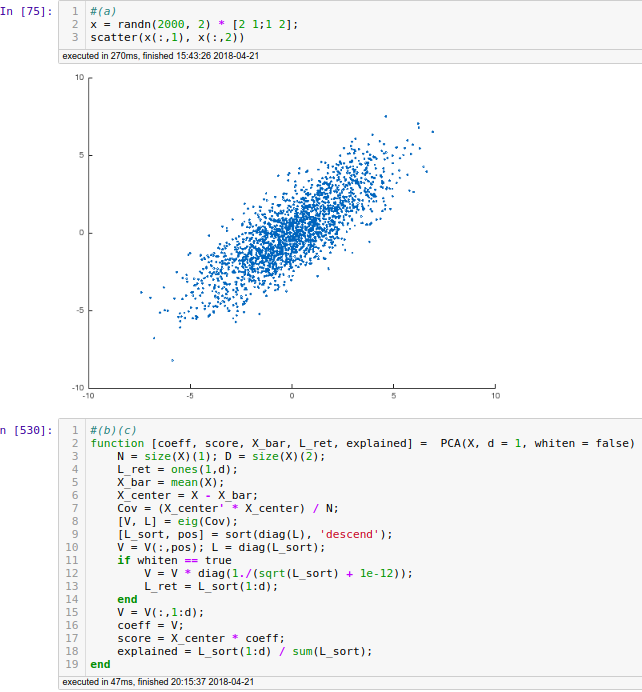
\includegraphics[width=1\textwidth]{2.jpg}\\
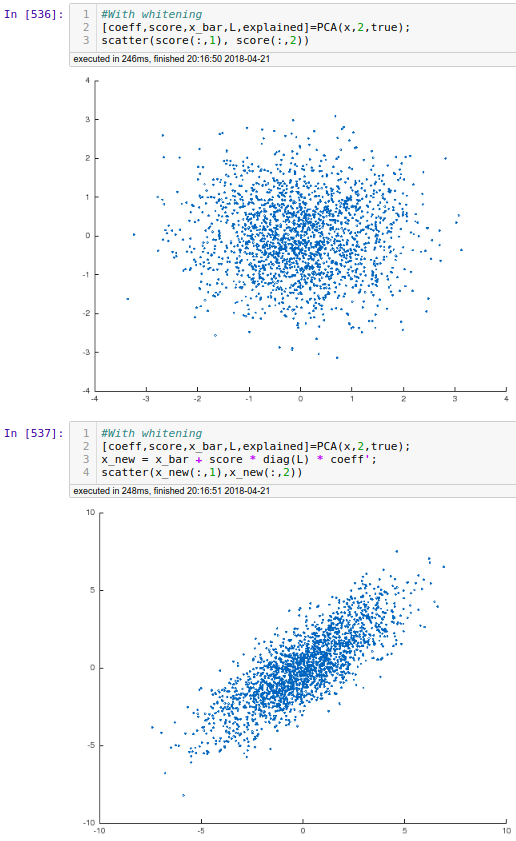
\includegraphics[width=1\textwidth]{3.jpg}\\
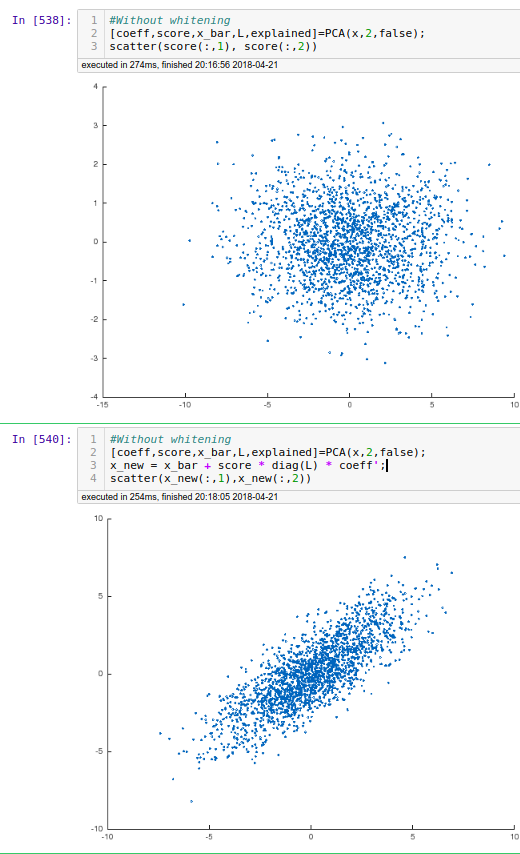
\includegraphics[width=1\textwidth]{4.jpg}\\
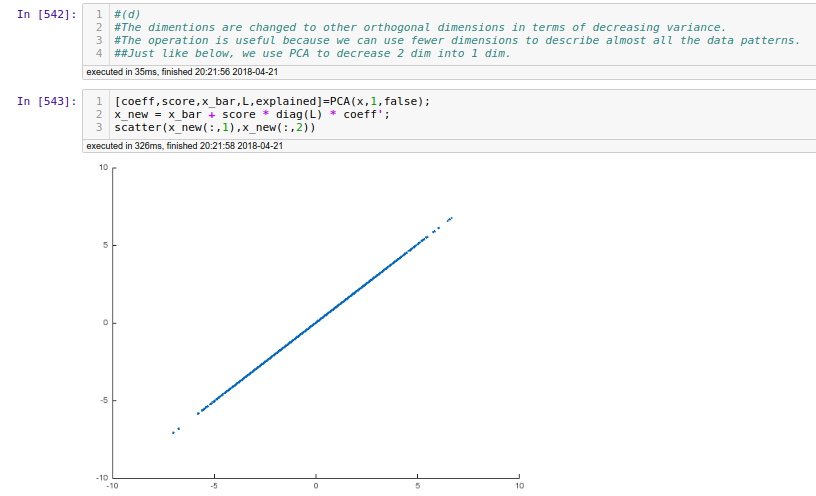
\includegraphics[width=1\textwidth]{5.jpg}\\
\end{solution}
% Add pairs of problems and solutions as needed

\end{document}
